\documentclass[a4paper,12pt,notitlepage]{report}
\usepackage[T1]{fontenc}    % Codifica dei font latini
\usepackage[utf8]{inputenc} % Lettere accentate da tastiera
\usepackage[english]{babel} % Lingua del documento  
\usepackage{graphicx}

\graphicspath{{images/}}    % Specifica la cartella con le immagini

\author{Matteo Colombo \and Andrea Troianiello}
\title{NonSoloLibri}



\usepackage{hyperref}       % Per collegamenti ipertestuali, 
\hypersetup{hidelinks}      % Rimuove riquadri dai collegamenti                     

\begin{document}


\begin{titlepage}           % Compone la pagina iniziale
    \centering
    {\Large DESIGN AND IMPLEMENTATION OF MOBILE APPLICATIONS}\\[4em]
    \includegraphics[width=7cm]{polimi.png}\\[8em]
    {\Huge NonSoloLibri}\\[4em]
    {\large MATTEO COLOMBO - ANDREA TROIANIELLO}\\[4em]
    \today
\end{titlepage}

\begin{abstract}            % Testo nella seconda pagina - riassunto
    \centering 
    Never loose a book again.\\ 
    Organize your book collection so that you always know where they are.\\

\end{abstract}

\tableofcontents            % Inserisce la tabella dei contenuti
\listoffigures              % Inserisce la lista delle figure
\listoftables               % Inserisce la lista delle tabelle

% ------------------------- % Inizio del contenuto
\chapter{Introduction}
\section{Purpose}
The purpose of this document is to describe all the aspect of the design and implementation of NonSoloLibri, a cross platform application whose aim is to help user managing their books collection.


\section{Scope}
NonSoloLibri is a small social network application designed for book enthusiast that allows them to organize and review their collection.\\
Users will be able to create libraries and to organize books in them.

Beside the storing functionality, NonSoloLibri has a social part that allows them to connect with other people with a friendship system.
Friends will be able to see the each other collections and wish-lists, so that they can surprise each other with presents.

A market place is be available, where every verified user will be able to sell or buy books.
\subsection{Goals}

\begin{enumerate}
    \item Allow the users to organize books in libraries.
    \item Allow the users to manage libraries and books.
    \item Allow the users to view their friends wishlist.
    \item Allow the users to sell and buy books in a market place.
\end{enumerate}


\section{Definitions, Acronyms, Abbreviations}

\subsection{Definitions}
\begin{description}
    \item[Cross-platform:] An application that runs on multiple operative systems, for example on both Android and iOS.
    \item[Flutter:] A cross-platform development SDK written in Dart, to develop for iOS, Android and Web.
    \item[Library:] A shelf characterized by a name, a photo and a list of books. 
    \item[Market Place:] A section of the application where users can sell and buy books.
    \item[Verified user:] A user whose identity has been verified by the system and is allowed to sell books in the market place.   
    \item[Widget:] A Flutter component that can represent anything, from a single layout item, to a whole page.
    \item[Wish-list:] A list of books that a user would like to acquire in the future. 
\end{description}


\subsection{Acronyms}
\begin{description}
    \item[API:] Application Programming Interface.
    \item[IEEE:] Institute of Electrical and Electronic Engineers.
    \item[SDK:] Software Development Kit. 
    \item[UML:] Unified Modeling Language. 
\end{description}
\subsection{Abbreviations}
\begin{description}
    \item[G.x:] The design goal number X.
    \item[R.y:] The design requirement number Y.
    \item[D.z:] The domain assumption number Z.  
\end{description}

\section{Reference Documents}
\begin{itemize}
    \item Android Developers website.
    \item Course slides.
    \item Firebase documentation.
    \item Flutter documentation.
    \item Material Design website. 
\end{itemize}

\section{Document Structure}
This document is divided in multuple chapters:
\begin{description}
    \item[Chapter 2-3:] Example
\end{description}
\chapter{Overall Description}

\section{Product Perspective}
NonSoloLibri will be developed from scratch and will be a mobile application that runs on
both iOS and Android. 

Data will be stored online so that they can retrieved from every device and to provide a sort of back-up option.
Thus, users will be required to have a smartphone or tablet and a Google account to sign in.

In the application the users will be able to make use of their device hardware to capture pictures of books and libraries or to scan the book barcodes.

Verifying users will be mandatory in order to let them access to the market place, to security layer and discourage bad behaviours.

\section{Actors}

We individuated three main actors for the application:

\begin{description}
    \item[Visitor] A person who has yet to login to the application and can only see the login page.
    \item[User] A visitor who successfully logged in into the application and can access to all the main feature of the aplication.
    \item[Verified User] An user who successfully verified himself and can access to the market place.
\end{description} 

\newpage

\section{Use Cases Diagram}
The main actors have different functionalities, according to the previous definitions. \\
The visitior can only perform the login, the user can also make other things, like to manage the library or review a book.
Verified user can interact with the market functions.\\
All the functions are shown using the following use case diagram:
\begin{figure}[!ht]
    \centering
	\includegraphics[scale=0.55]{images/use-case-diagram.png}
	\caption{Use case diagram}
	\label{fig:usecasediagram}
\end{figure}

\section{Product Requirements}
\begin{enumerate}
    \item Visitors should be able to login with their Google account.
    \item Users should be able to create libraries.
    \item Users should be able to edit libraries.
    \item Users should be able to customize libraries with photos or images.
    \item Users should be able to delete libraries.
    \item Users should be able to view libraries.
    \item Users should be able to add books to libraries.
    \item Users should be able to delete books from libraries.
    \item Users should be able to move books from a library to another.
    \item Users should be able to view books information.
    \item Users should be able to create books if they are not present in the database.
    \item Users should be able to suggest changes to books information.
    \item Users should be able to search for books in the database.
    \item Users should be able to send friendship requests.
    \item Users should be able to manage friendships.
    \item Users should be able to create a wish list.
    \item Users should be able to view their friends wish lists.
    \item Users should be able to verify themself.
    \item Verified users should be able to access to the market place.
    \item Verified users should be able to buy books in the market place.
    \item Verified users should be able to sell books in the market place.
\end{enumerate}

\section{Constraints}

\subsection{Hardware  and Software Constraints}
\begin{enumerate}
    \item To use the application, users are required to have a smartphone or a table. The device can have either Android or iOS 
        \begin{itemize}
            \item For Android the minimum supported versione is Android 5.0 Lollipop.
            \item For iOS the minimium supported version is iOS 10.
        \end{itemize}
    \item The application requires a device configured and able to connect to the Internet.
    \item The application requires a device with a photocamera.
\end{enumerate}

\subsection{Safety and Regulation Constraints}
\begin{enumerate}
    \item The system must guarantee data is protected and accessible only by its owner.
    \item The application must ask for user permissions to acquire, store and elaborate images from their devices.
    \item The system must complain with local laws.  
\end{enumerate}


\section{Domain assumptions}
\begin{enumerate}
    \item Administration tasks such as verification of the users and data checks on books inserted by users are made through an independent web-application whose design is not part of this document.
    \item Users should behave coherently and in respect of good manners.
    \item Users should type in correct information when adding a new book.
    \item A library is composed by: a name, a picture or an image and can be favourite or not.    
    \item A library can contain only one copy of a book.
    \item Multiple books with the same ISBN code can be located in different libraries.
    \item A book is characterized by: title, authors, publisher, release date, length, edition number, price and a ISBN code.
    \item The application will work as an intermediary between users for book trading, but transactions and shipment will happen outside of the application context.
\end{enumerate}


\chapter{Architectural Design}
\section{Overview}
This chapter focuses on the architectural structure, components will be described explaining how they interact with each other.
The system will be illustrated both physically and logically.\\
The main high level components of the system are the following:\\
\begin{itemize}
    \item
    \textbf{Applicaton device:} User's device where the application is installed. This application implements most of the logic of the system.
    \item
    \textbf{Cloud server:}  The server side of the system is responsible for the data storage and sync.\\ This layer contains a NoSQL database is used, 
    which stores data in flexible, JSON-like documents. The main keys are flexiblility, expressive querying, realtime updates, offline support and scalability.\\
    \item
    \textbf{Applicaton web:} A pre-existing application used by responsibles that allows to check and edit the stored data.
\end{itemize}
\clearpage
\section{Component View}
\subsection{High-Level Component View}
\begin{figure}[!h]
    \centering
    \includegraphics[scale=0.5]{images/high-level-component-view.png}
    \caption{High level component diagram}
    \label{ref:highlevelcomponentdiagram}
\end{figure}
This component diagram displays the high-level view of the sistem focusing on application device.
The component developed are:
\begin{itemize}
    \item
    \textbf{Application:} It is the core of the system, it manages all information provided by the others services
     and performs the majority of the functions. It provides the client access to the entire system.
    \item
    \textbf{Firestore:} This component has an account manager and backup roles. It receives the data from the application and provides them when necessary.
\end{itemize}
Moreover, application is integrated with \textbf{Google Sign In}, which provides the authatication functions of the system, 
using directly the credetial of Google.
\clearpage
\subsection{Application}
\begin{figure}[!h]
    \centering
    \includegraphics[scale=0.4]{images/application-component-diagram.png}
    \caption{Application component diagram}
    \label{ref:applicationcomponentdiagram}
\end{figure}
\begin{itemize}
    \item
    \textbf{Model:} It represents how the data are structured in the application and ready to be stored by Firestore.
    \item
    \textbf{Home:} Is is the entry point of the application. Creates the Localization and LibProvider components. Handles login parts and the choice of the library.
    \item
    \textbf{Localization:} It setups the language of the application based on the language of the OS.
    \item
    \textbf{LibProvider:} Provides LibraryRepo, BookRepo,Auth, BarcodeScanner and ImagePicker.
    \item
    \textbf{LibraryRepo:} This components is used to communicate with Firebase and to manage the library collection.
    \item
    \textbf{BookRepo:} It communicates with Firebase and saves an retrives the data of the book.
    \item
    \textbf{Auth:} This components is used to handle the authentication phase of the user.
    \item
    \textbf{BarcodeScanner:} It uses the camera the ISBN from the barcode of a book.
    \item
    \textbf{ImagePicker:} It uses the library that allows to take a photo with camera or pick an image from the gallery of the device.
    \item
    \textbf{LibraryPage:} It is the union of widgets that shows the books that belong to a given library.
    \item
    \textbf{BookPage:} It handles the infromation of the book, its reviews and the associated offers by the users. 
    \item
    \textbf{Search:} Shows a list of the books, which match with a user's input.
    \item
    \textbf{User:} It is the group of pages and widget that handles the profiles management, including friendships and conversation between users.
\end{itemize}
\clearpage
\section{Relationship between the model and the database}
During the design of the application has been used a database first approach. The database was the core during the design and the model was derived from it 
respecting the existing relationships between the entities.\\
The following there is the ER digram used to implements the database:
\begin{figure}[!h]
    \centering
    \includegraphics[scale=0.43]{images/er-diagram.png}
    \caption{ER diagram}
    \label{ref:erdiagram}
\end{figure}
\begin{itemize}
    \item
    \textbf{Books:} Collects all information of the books contained in the database. Each book is characterized  by a ISBN, which is its primary key, and other information including a title, a description and a image.
    \item
    \textbf{Users:} The users use the login function of the application. The id is generated automatically, the name and email are saved, but the password no.
    \item
    \textbf{Libraries:} The libraries created by each user.
    \item
    \textbf{Reviews:} Includes a score and a comment wrote by a user associated to a book.
    \item
    \textbf{Authors:} Contains the main of information of the creator of one or more books.
    \item
    \textbf{Requests:} Contains all suggestions made by a user to edit the book information. The idetifier is the union of the ISBN of the book and the user's id.
    \item
    \textbf{Market:} Collects the sales offers of books made by each user.
    \item
    \textbf{Conversations:} The discussion between two or more users.
    \item
    \textbf{Messages:} The texts exchanged during a conversation.
\end{itemize}
During the implementation, we have opted for the introduction of data duplication. This allows to yield the main characteristics of the document-oriented database.



\chapter{Interface Design}
\section{UX Diagram}
This diagram describes in detail all the pages of the application, how the application can
be navigated including the screens, the input forms and the possible errors.\\

\begin{figure}[!ht]
    \centering
	\includegraphics[scale=0.39]{images/ux-diagram.png}
	\caption{UX diagram}
	\label{fig:uxdiagram}
\end{figure}
\clearpage

\section{User Interfaces Design}
The following images are the most important pages of the application.\\
\begin{figure}[!htb]
    \begin{minipage}[b]{0.3\textwidth}
        \includegraphics[scale=1]{images/login-page.png}
        \caption{Login}
        \label{ref:loginpage}
    \end{minipage}
    \hfill
    \begin{minipage}[b]{0.3\textwidth}
        \includegraphics[scale=1]{images/libraries-page.png}
        \caption{Libraries}
        \label{ref:librariespage}
    \end{minipage}
    \hfill
    \begin{minipage}[b]{0.3\textwidth}
        \includegraphics[scale=1]{images/search-page.png}
        \caption{Search}
        \label{ref:search}
    \end{minipage}
\end{figure}
The entry point of the application is login page (Figure \ref{ref:loginpage}), 
where the user insert his Google credentials.\\ 
After, the page with the list of libraries is displayed. 
Each library can be edited or deleted.In this page there are a icon button, 
that allows to search through all the books contained in the database (Figure \ref{ref:search}), 
and a floating button, for the creation of a new library.\\
\clearpage
\begin{figure}[!htb]
    \begin{minipage}[b]{0.3\textwidth}
        \centering
        \includegraphics[scale=1]{images/menu.png}
        \caption{Menu}
        \label{ref:menu}
    \end{minipage}
    \hfill
    \begin{minipage}[b]{0.3\textwidth}
        \centering
        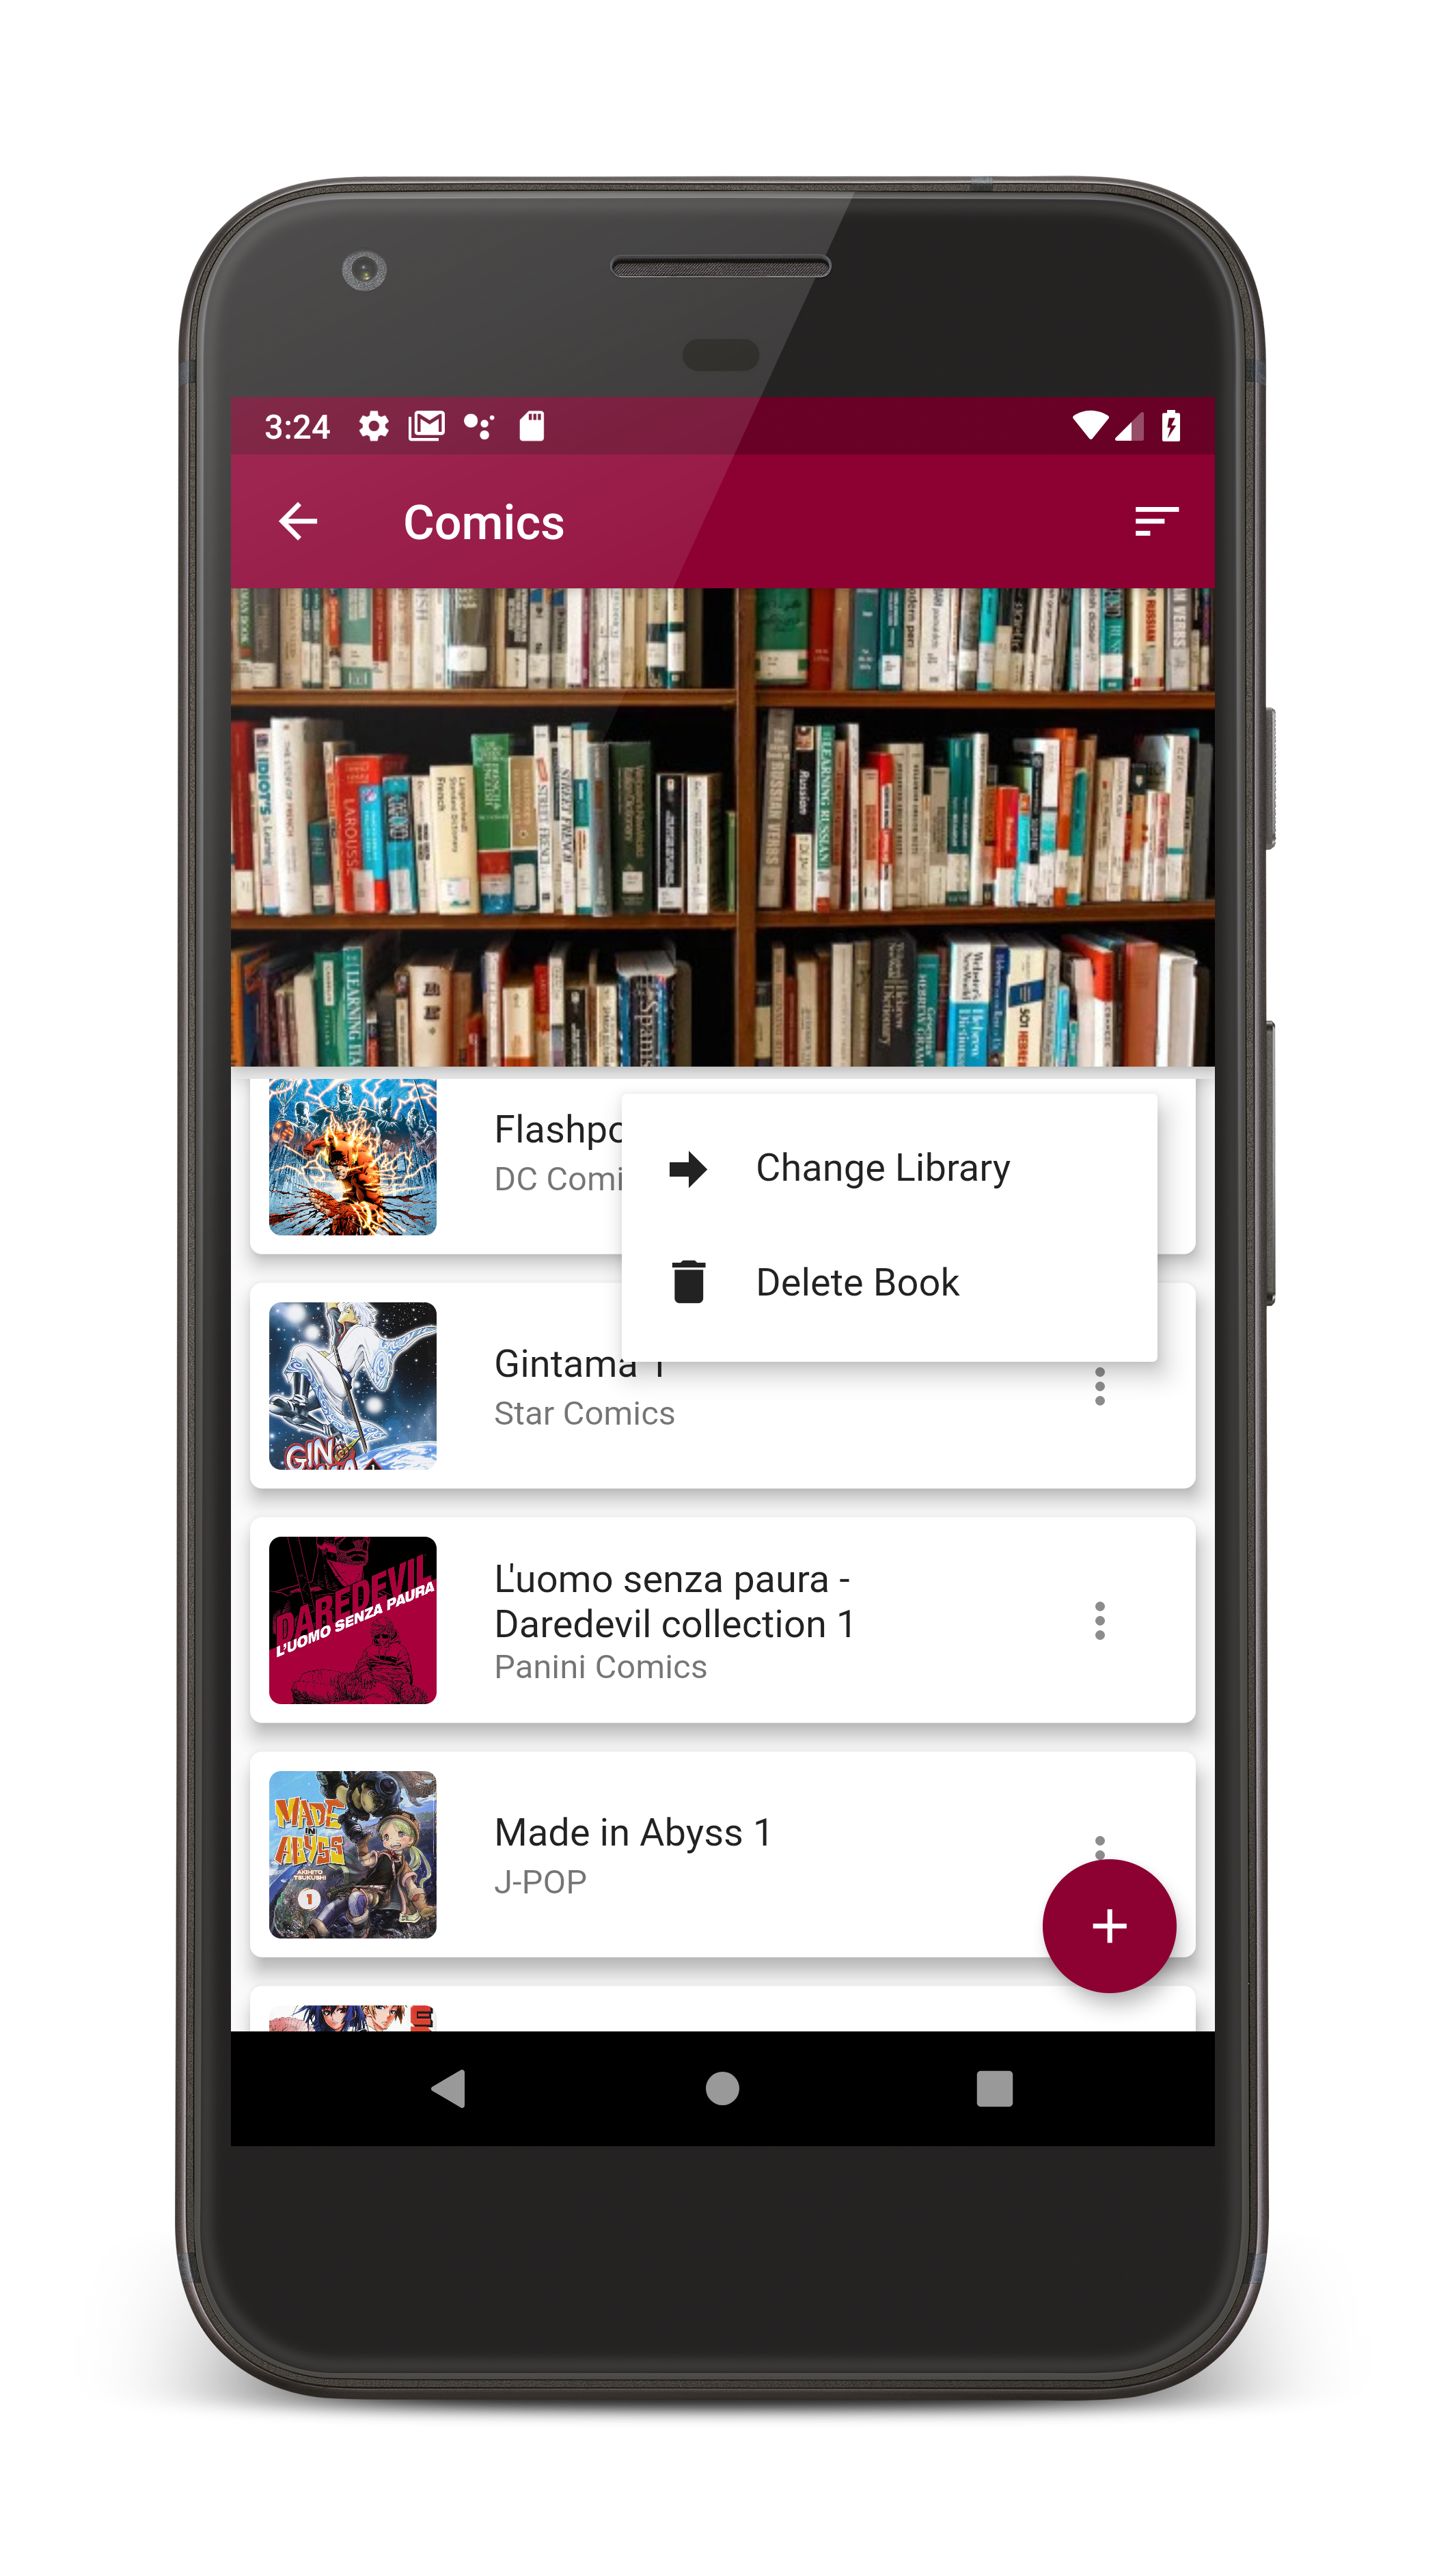
\includegraphics[scale=1]{images/library-page.png}
        \caption{Library}
        \label{ref:librarypage}
    \end{minipage}
    \hfill
    \begin{minipage}[b]{0.3\textwidth}
        \centering
        \includegraphics[scale=1]{images/add-new-book-dialog.png}
        \caption{New book}
        \label{ref:addnewbook}
    \end{minipage}
\end{figure}
From the libraries page, can be opened a menù (Figure \ref{ref:menu}), which allows to reach the application settings, 
account functionalities and to log out.\\ After opened a library, 
all of the book contained are displayed (Figure \ref{ref:librarypage})and each of them moved to a another library or deleted.\\ 
The floating buttton opens the camera that reads the ISBN of the book and automatically add it. 
If it doesn’t exists, a dialog, that allows to insert a new book, is opened.
\clearpage
\begin{figure}[!htb]
    \begin{minipage}[b]{0.3\textwidth}
        \centering
        \includegraphics[scale=1]{images/book-info-page.png}
        \caption{Book info}
        \label{ref:bookinfo}
    \end{minipage}
    \hfill
    \begin{minipage}[b]{0.3\textwidth}
        \centering
        \includegraphics[scale=1]{images/no-review.png}
        \caption{No review}
        \label{ref:noreview}
    \end{minipage}
    \hfill
    \begin{minipage}[b]{0.3\textwidth}
        \centering
        \includegraphics[scale=1]{images/reviews-page.png}
        \caption{Reviews}
        \label{ref:reviewspage}
    \end{minipage}
\end{figure}
The book page (Figure \ref{ref:bookinfo}) uses a tab bar to display all information releated to the book.\\ 
The first one contains the specific information, like the title, image of the cover, list of author and description.\\ 
The second one (Figures \ref{ref:noreview} and \ref{ref:reviewspage}) lists all reviews. This section is divided in two parts.\\
The fist part shows the review wrote by the user, if no exists allows to write it, otherwise displays it and, using a button, allows to edit it.\\
The second part shows a scrollable list of reviews wrote by other users and can be filtred based on the scores.
\clearpage
\section{Hardware Interfaces}
This project doesn’t require any hardware interface.
\section{Software Interfaces}
\begin{itemize}
    \item Database Management System (DBMS):
    \begin{itemize}
        \item 
        Name: Cloud Firestore
        \item 
        Source: https://firebase.google.com/products/firestore/
    \end{itemize}
    \item Storage:
    \begin{itemize}
        \item 
        Name: Cloud Storage
        \item 
        Source: https://firebase.google.com/products/storage
    \end{itemize}
    \item Server:
    \begin{itemize}
        \item 
        Name: Cloud Functions
        \item 
        Source: https://firebase.google.com/products/functions/
    \end{itemize}
    \item
    Operiting systems:
    \begin{itemize}
        \item 
        Name: Android
        \item 
        Minimum version: 5.0 Lollipop 
        \item 
        API level: 21
        \item 
        Source: https://www.android.com/\\ 
        \item 
        Name: iOS
        \item 
        Minimum version: 10
        \item 
        Source: https://www.apple.com/ios
    \end{itemize}
\end{itemize}
\section{API Interfaces}
The application communicates with the database on Firebase using:
\begin{itemize}
    \item
    firebase\_core (version 0.4.0+8), a Flutter plugin to use the Firebase Core API, which enables connecting to multiple Firebase apps.
    \item
    firebase\_analytics (version 4.0.2), allows to use the Google Analytics for Firebase API, a free app measurement solution that provides insight on app usage and user engagement.
    \item
    firebase\_auth (version 0.14.0), a plugin to use the Firebase Authentication API, that aims to make building secure authentication systems easy, while improving the sign-in and onboarding experience for end users. It provides an end-to-end identity solution, supporting email and password accounts, phone auth, and Google, Twitter, Facebook, and GitHub login, and more.
    \item
    cloud\_firestore (version 0.12.9), a library that allows to communicates with the NoSQL cloud database of Google (Firestore).
    \item
    firebase\_storage (version 3.0.5), a Flutter plugin to use the Cloud Storage API. Cloud Storage is used to upload images or other files on Firebase.
\end{itemize}
During the adding new book phase, the ISBN is read using the barcode, that allowed by flutter\_barcode\_scanner (version 0.1.5+1).
\\
\\
For the user's login, the system uses the Google Sign In API. This API provides the authentication of the user and retrives his main information (name and email).
The used libraries are google\_sign\_in (version 4.0.6) and firebase\_auth.
\\
\\
The plugins intl (version 0.15.8) and intl\_translation (version 0.17.3) are used to generate and manage the language of the application, according to the language of the OS.
\chapter{Implementation and Test Planning}

\section{Implementation}
For the client, the application has been implemented using Flutter, an SDK that simplifies cross-platform development and allows to write Dart code
that can be compiled into native languages without loss of performances. Thanks to flutter we were able to write in only one language but to support two,
different, operative systems.

For the backend it was decided to use Firebase to simplify the design and to take benefit of the infrastructure provided by Google,
that offers both reliability and security.

Before the development, the application was divided in various components - called Widgets, in Flutter - that could be developed independently and a bottom up approach was choosen.
Furthemore, the design of the application was thought with flexibility in mind, and the core of the application is completely independent from external
libraries such those to access to hardware of the device, or those that implement the database.

At the moment of writing this document, all the features related to organizing a user library were implemented, while those related to the social network 
aspect of the application and to the market-place are yet to be implemented.

\newpage
\section{Testing}
The application has been tested using the native tools provided by both Firebase and Flutter.

For firebase, the testing tools provided by the Firebase console were used. In this way we were able to test users permissions and API calls, that were later used in the application.

For Flutter the library \emph{flutter\_test}, which is provided by the Flutter SDK, was used, together with \emph{mockito}, an external library that simplifies mocking of dependences.

\emph{Flutter\_test} was used to generate unit, widget and integration tests, that were used to test single functionalities and to test together the various widget that compose the pages.

\emph{Mockito} was used to create mocks of external libraries that can not be tested within the application such as the photo camera, the barcode scanner and the Firebase implementation.
With this approach we were able to test most of the implementation.

In addition, extensive tests were made by real users, by testing the application in daily conditions with both physical devices and emulators.
% ------------------------- % Fine del contenuto

\begin{thebibliography}{9}
    \bibitem{pantieri:arte}
    Pantieri, Lorenzo e Tommaso Gordini (2017),
    \emph{L’arte di scrivere con \LaTeX},
    \url{http://www.lorenzopantieri.net/LaTeX_files/ArteLaTeX.pdf}.
\end{thebibliography}
    

\end{document}